%=====================================================================
%  ZeoAuction — Timeline Chart + Task Board Screenshots
%  Web Services & Service-Oriented Architecture — M.Sc. IT (Sem 3)
%
%  UPLOAD THESE 4 IMAGES TO OVERLEAF WITH THESE EXACT NAMES:
%     zeoauction_timeline.png
%     zeoauction_timeline1.png
%     zeoauction_calender.png
%     zeoauction_backlog.png
%  Compile with pdfLaTeX.  Output: 1 summary page + 4 image pages.
%=====================================================================

\documentclass[10pt,a4paper]{article}

\usepackage[T1]{fontenc}
\usepackage[utf8]{inputenc}
\usepackage[margin=1.7cm,top=1.5cm,bottom=1.5cm]{geometry}
\usepackage{lmodern}
\usepackage{graphicx}
\usepackage{booktabs}
\usepackage{array}
\usepackage[table]{xcolor}
\usepackage{titlesec}
\usepackage{caption}
\usepackage[hidelinks]{hyperref}

\definecolor{accent}{HTML}{1F4E79}

\titleformat{\section}{\normalsize\bfseries\color{accent}}{\thesection.}{0.5em}{}
\titlespacing*{\section}{0pt}{8pt}{3pt}

\captionsetup{font=small,labelfont={bf,color=accent}}
\setlength{\tabcolsep}{4pt}
\renewcommand{\arraystretch}{1.12}
\setlength{\parindent}{0pt}
\setlength{\parskip}{4pt}
\pagestyle{empty}

\newcommand{\hdr}[1]{\textcolor{white}{\bfseries #1}}
\newcommand{\hdrrow}{\rowcolor{accent}}

\begin{document}

%=====================================================================
% PAGE 1 — TITLE PAGE
%=====================================================================
\begin{titlepage}
\centering
\vspace*{2.2cm}

{\Huge\bfseries\color{accent} ZeoAuction\par}
\vspace{0.5cm}
{\Large Distributed Real-Time Auction Platform\par}
\vspace{0.35cm}
{\large A Microservices / Service-Oriented Architecture Project\par}

\vspace{1.5cm}
\rule{0.75\textwidth}{1pt}\par
\vspace{0.6cm}
{\LARGE\bfseries Task Timeline, Milestones\\[0.25cm] and Team Task Assignments\par}
\vspace{0.6cm}
\rule{0.75\textwidth}{1pt}\par

\vspace{1.5cm}
{\large\bfseries Subject:} Web Services \& Service-Oriented Architecture\\[0.28cm]
{\large\bfseries Programme:} M.Sc.\ Information Technology (Semester 3)\\[0.28cm]
{\large\bfseries Submission:} Group Project --- Team of 8\\[0.28cm]
{\large\bfseries Project Window:} 03 August 2026 --- 20 November 2026 (16 weeks)\\[0.28cm]
{\large\bfseries Planned Effort:} 1{,}600 person-hours (200 hours per member)

\vspace{1.6cm}
\begin{tabular}{ll}
\toprule
\textbf{Member} & \textbf{Enrolment ID} \\
\midrule
Naitik   & 202512006 \\
Sumit    & 202512124 \\
Sagar    & 202512107 \\
Harshal  & 202512013 \\
Jaydip   & 202512090 \\
Gaurang  & 202512007 \\
Jay      & 202512123 \\
Ayush    & 202512084 \\
\bottomrule
\end{tabular}

\vfill
{\large August 2026}
\end{titlepage}

\clearpage

%=====================================================================
% PAGES 2–5 — FIGURES, ONE PER PAGE
%=====================================================================

\begin{center}
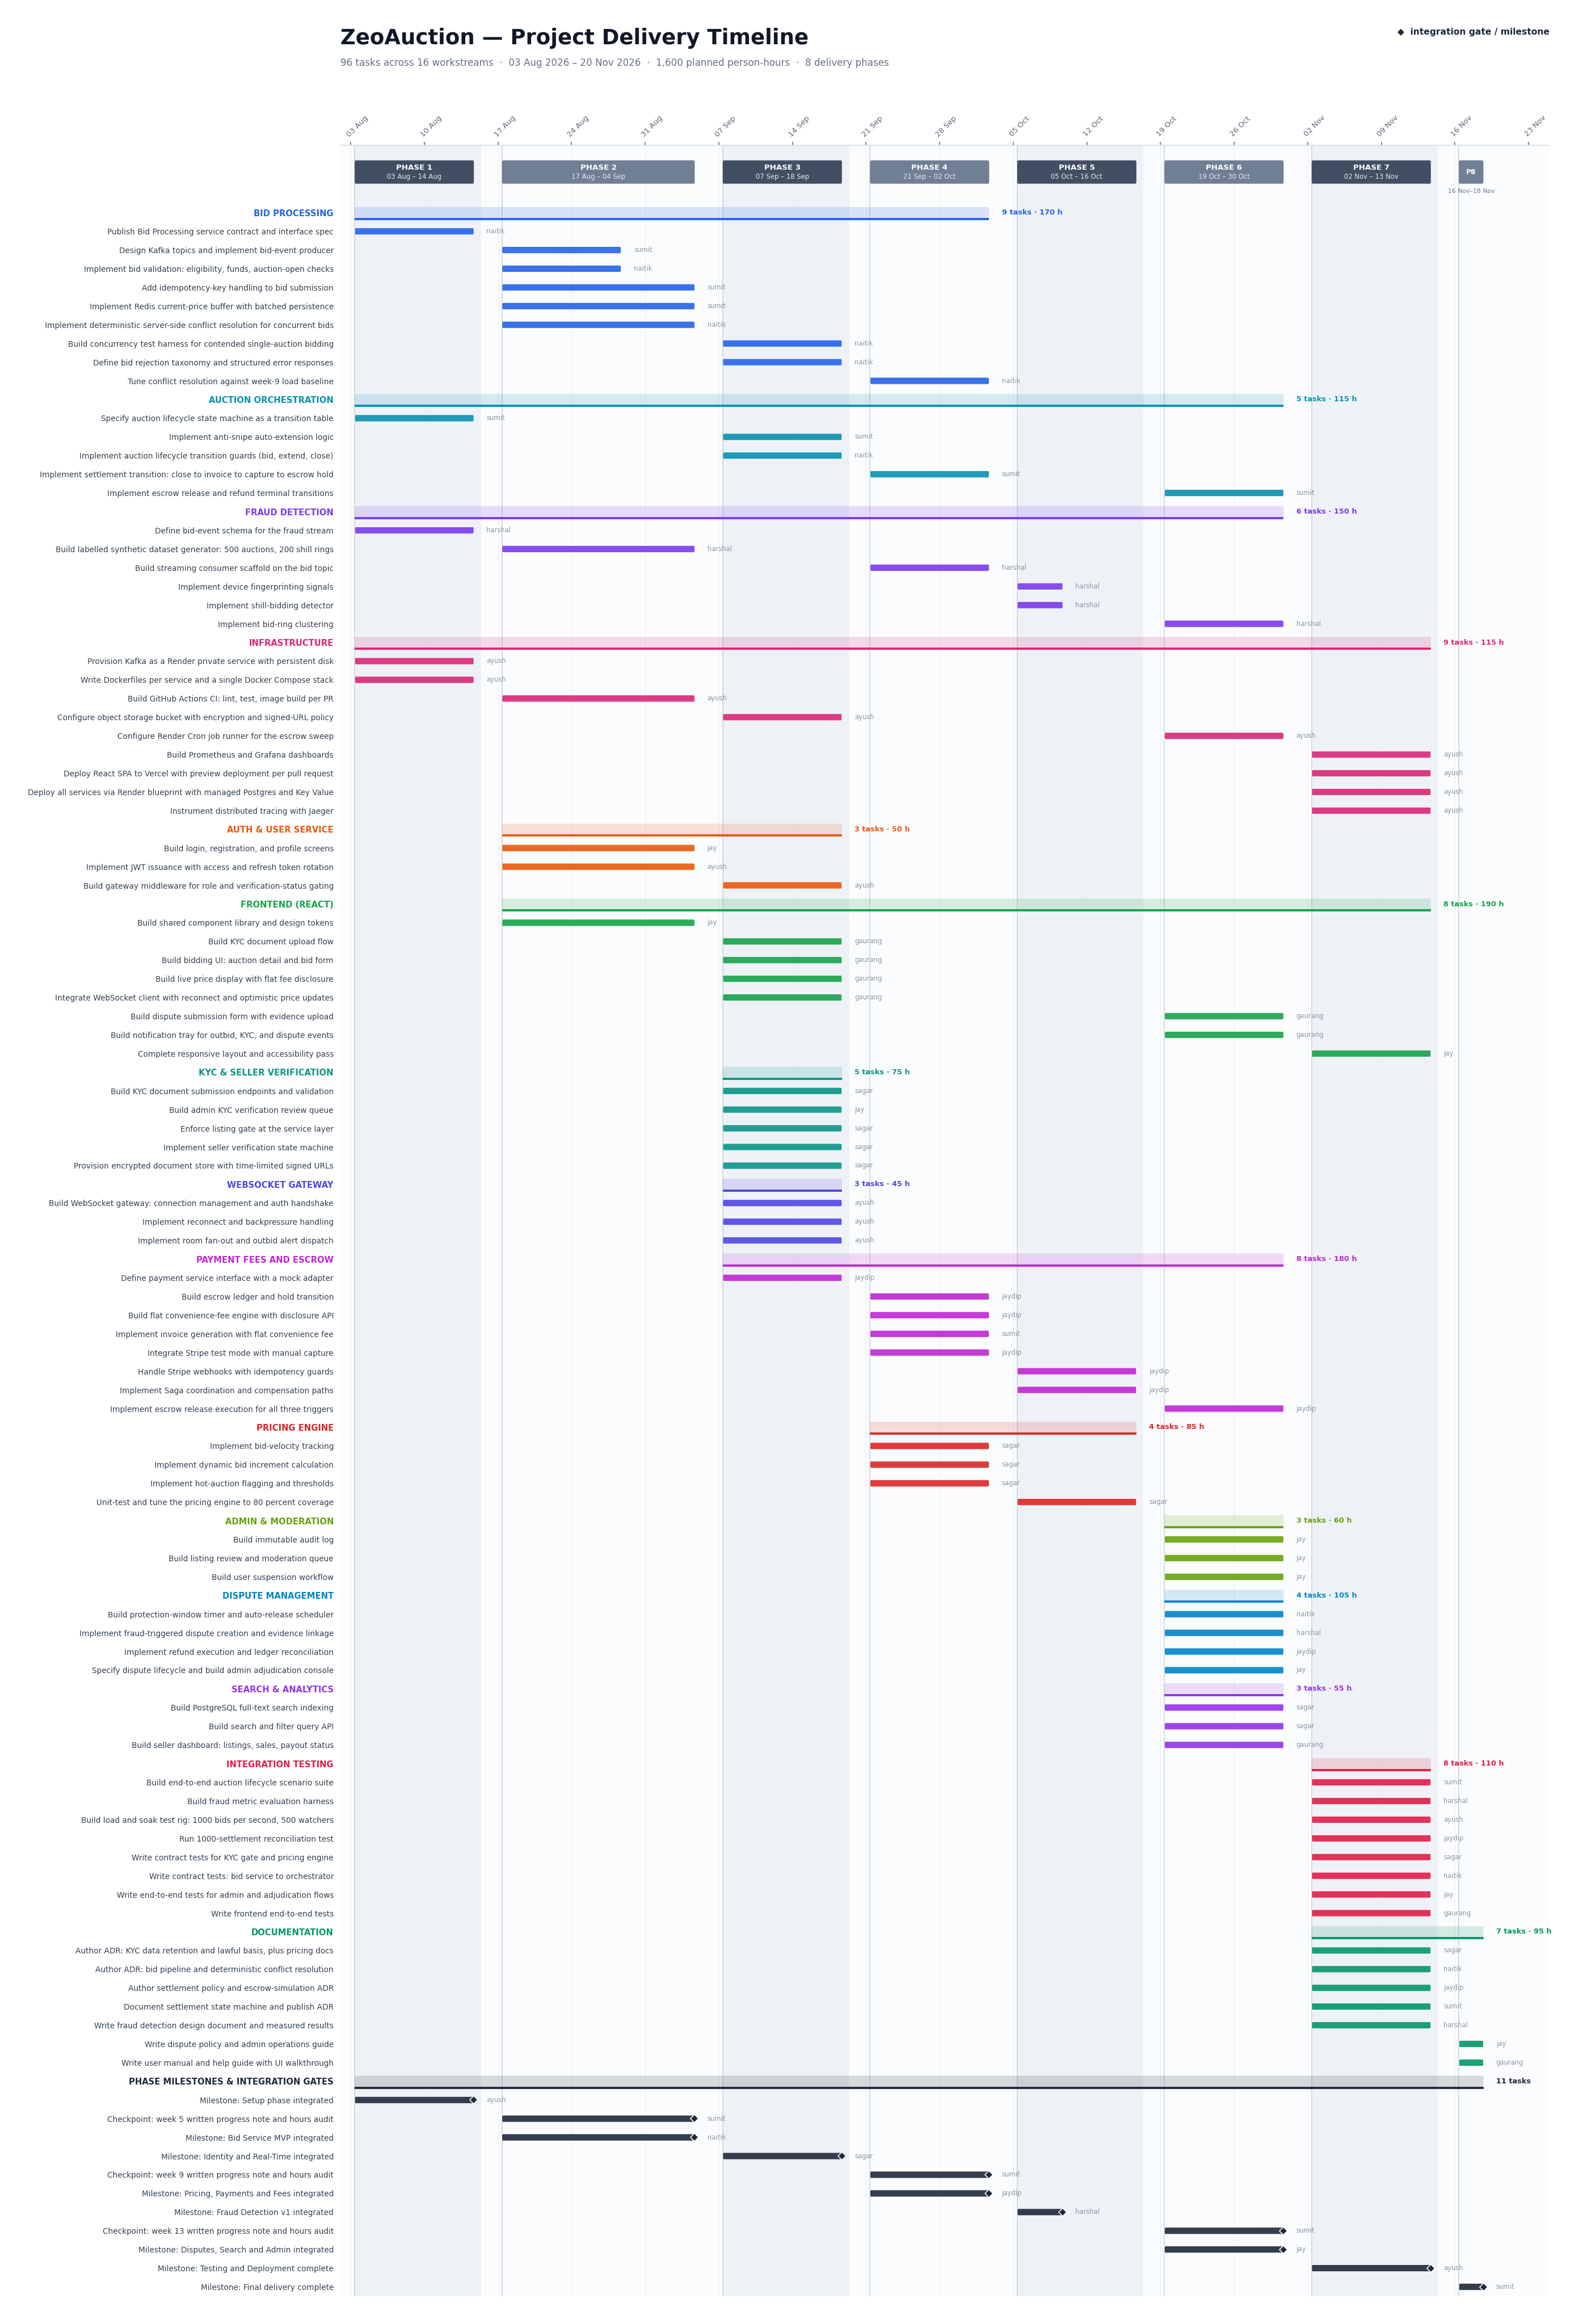
\includegraphics[width=\textwidth,height=0.92\textheight,keepaspectratio]{zeoauction_timeline.png}
\captionof{figure}{Project delivery timeline --- 96 tasks across 16 workstreams and 8 phases, with
the assigned member against each bar and integration gates on the milestone track.}
\end{center}
\clearpage

\begin{center}
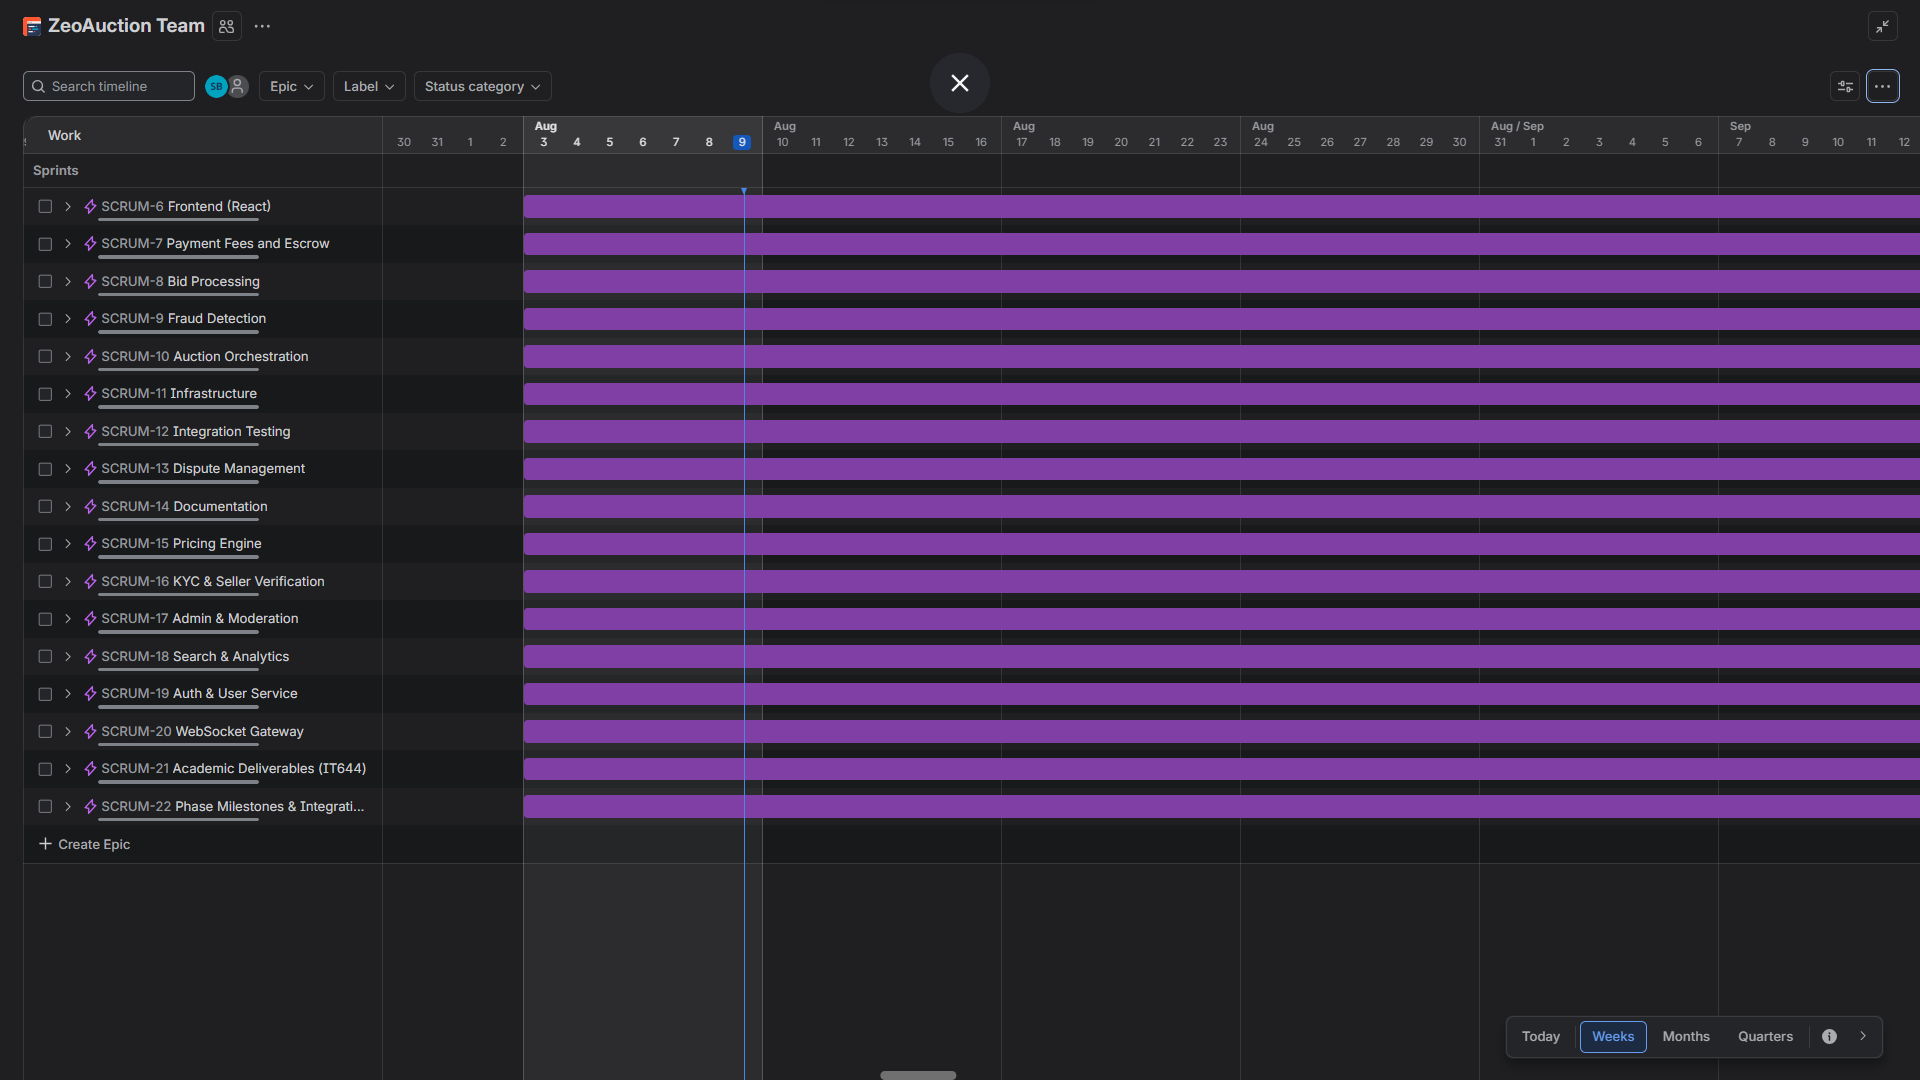
\includegraphics[width=\textwidth,height=0.92\textheight,keepaspectratio]{zeoauction_timeline1.png}
\captionof{figure}{Jira timeline view --- epic-level schedule across the project window.}
\end{center}
\clearpage

\begin{center}
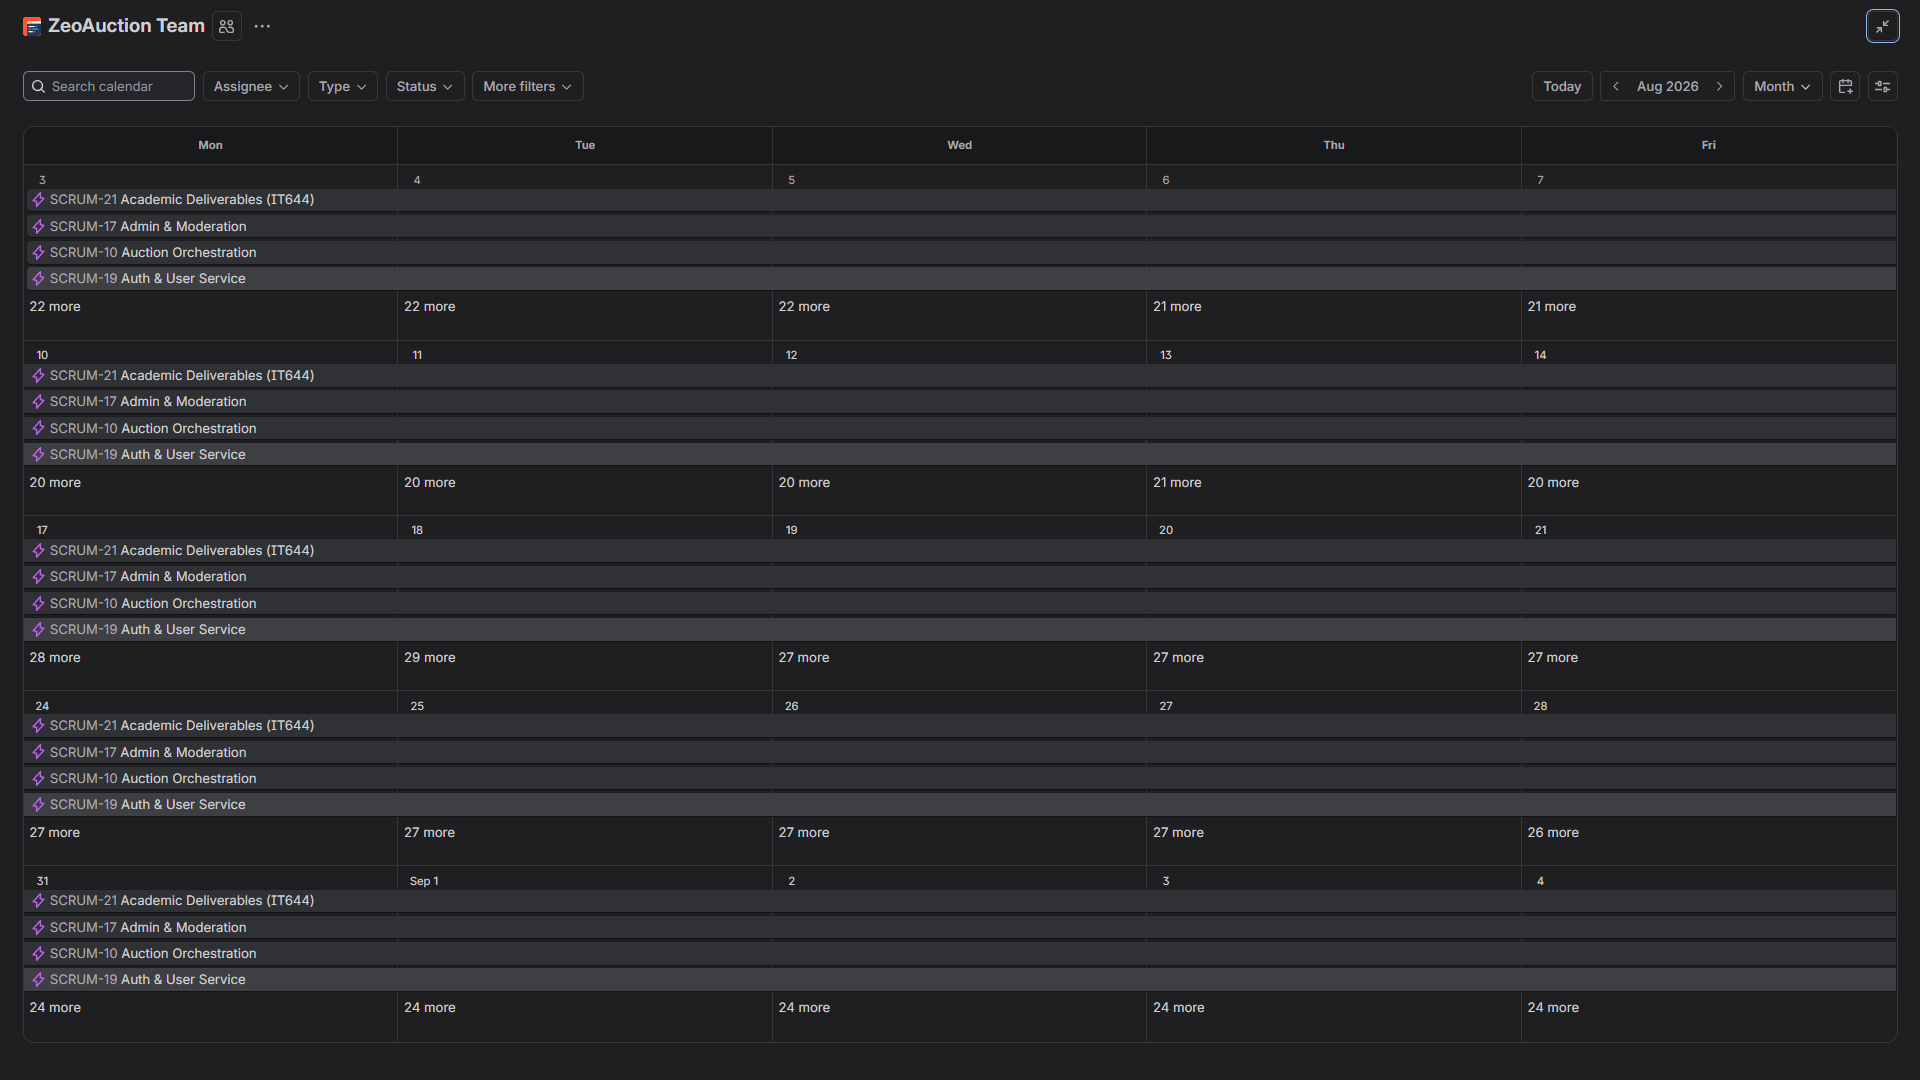
\includegraphics[width=\textwidth,height=0.92\textheight,keepaspectratio]{zeoauction_calender.png}
\captionof{figure}{Jira calendar view --- task due dates across the sixteen-week schedule.}
\end{center}
\clearpage

\begin{center}
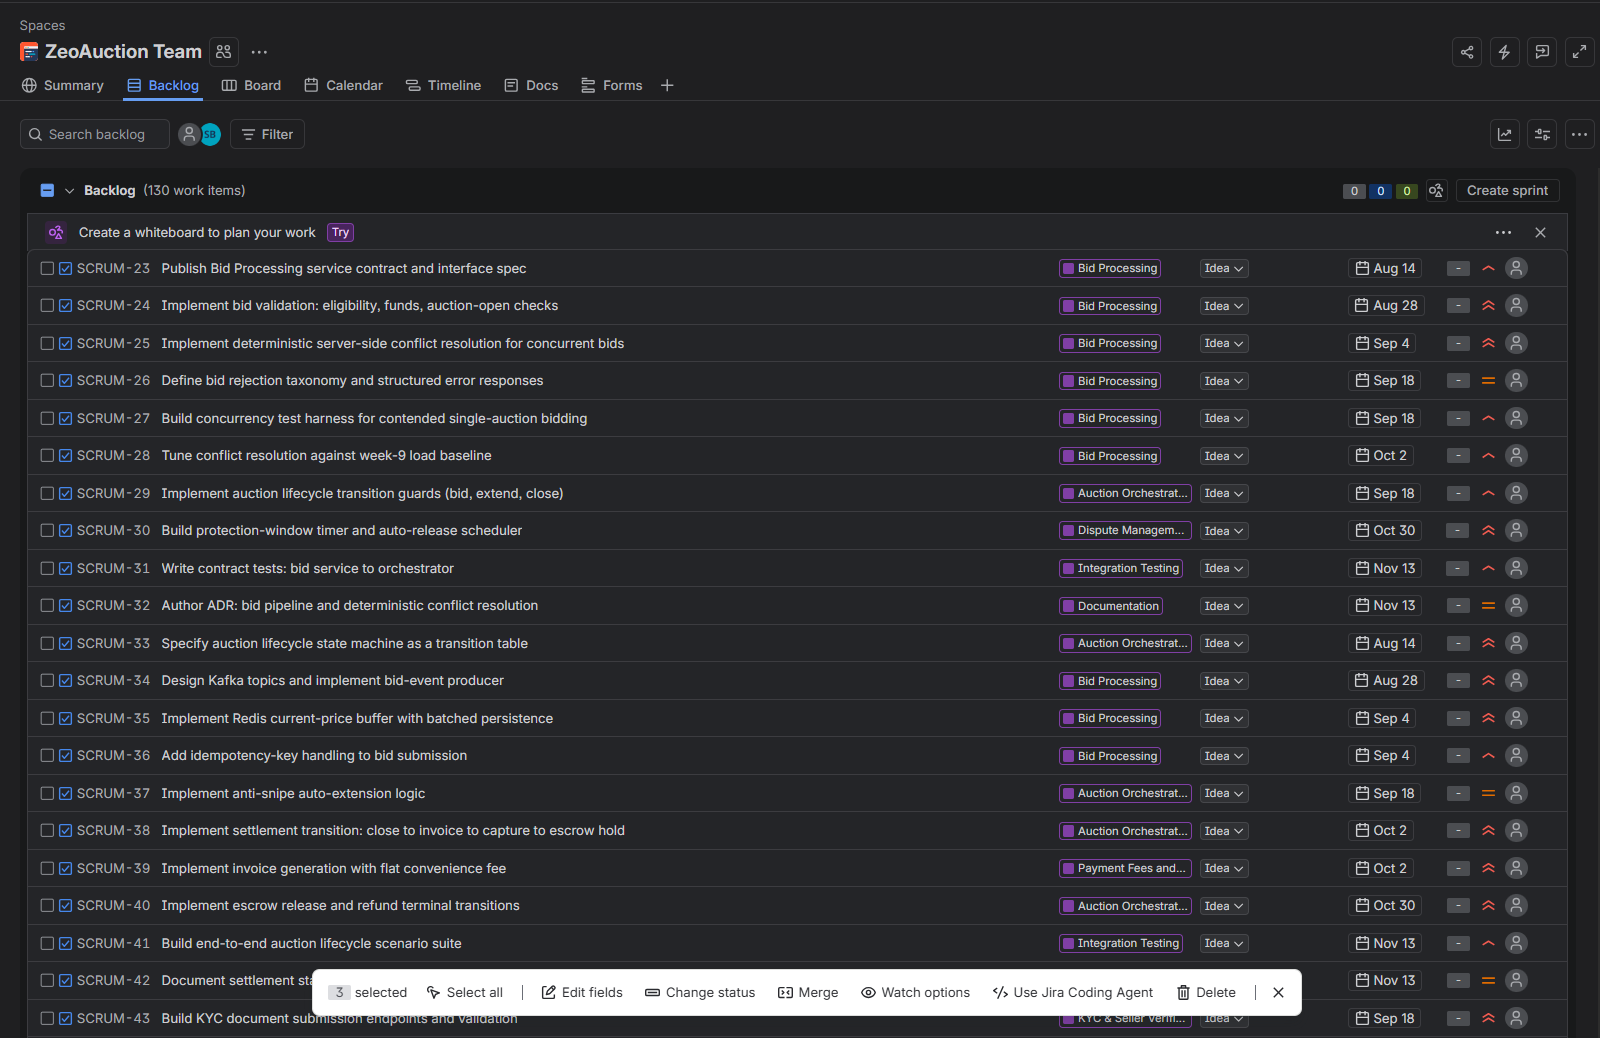
\includegraphics[width=\textwidth,height=0.92\textheight,keepaspectratio]{zeoauction_backlog.png}
\captionof{figure}{Jira backlog --- work items tagged by workstream component, each with an assignee,
priority and a due date aligned to its delivery phase.}
\end{center}

\end{document}